\documentclass[a4paper,8pt]{article}
\usepackage[margin=1.5cm]{geometry}
\usepackage{graphicx}
\usepackage{marvosym}
\begin{document}
\title{Operating Systems and Application Software}
\author{Ale}
\maketitle
\section{Operating Systems}
The set of program instructions that tell the computer what to do is known as
\textbf{software}. It can be classified into two basic categories:
\begin{itemize}
\item the \textbf{system software}, which includes all the programs that control
  the basic functions of a computer. (e.g. operating systems, programming 
  software, device drivers and utilities.)
\item the \textbf{application software}, which comprises programs that let you
  perform specific tasks. Typical applications include \textsl{word processing},
  databases, \textsl{spreadsheets}, educational programs, email 
  and video games.
\end{itemize}
The \textbf{operating system} is a set of programs that control the hardware and
software resources of a computer system.\\
It acts as an interface between the user and the computer.
Typical functions of the OS include handling input/output operations, 
running programs and organizing files on disks.
\subsection{Graphical User Interface (GUI)}
The term \textbf{user interface} refers to the standard procedures that the user
follows in order to interact with a computer. In the late 1970s and early 80s,
the way users accessed computer system was very complex. They had to memorize
and type a lot of commands just ot see the contents of a disk, to copy files
or to respond to a single prompt. In fact, it was only experts who used 
computers, so there was no need for a user-friendly interface.\\
In 1984, Apple produced the Macintosh, the first computer with a mouse and a
\textbf{graphical user interface (GUI)}. Macs were designed with one clear aim:
to facilitate interaction with the computer. A few years later, Microsoft 
launched Windows, another operating system based on graphics and intuitive
tools. Nowadays, computers are used by all kinds of people, and as a result
there is a growing emphasis on accessibility and user-friendly systems.\\
A \textbf{GUI} makes use of a \textbf{WIMP} environment: windows, icons, menus
and pointer. The background of the screen is called the \textbf{desktop}, which 
contains labelled pictures called \textbf{icons}. These icons represent
\textbf{files} or \textbf{folders}. Double-cliking a folder opens a window
which contains \textbf{programs, documents}, or more nested folders. When
you are in a folder, you can launch a program or document by double-clicking 
the icon, or you can drag it ot another location. When you run a program, 
your PC opens a window that lets you work with different tools.
All the programs have a high level of consistency, with similar toolbars,
menu bars, buttons and dialog boxes. A modern OS also provides access to 
networks and allows multitasking, which means you can run several programs - 
and do various tasks - at the same time.
The most popular operating systems are:
\begin{itemize}
\item The \textbf{Windows} family - designed by Microsoft and used on most PCs.
  The most recent version is Windows 8.
\item \textbf{Mac OS X} - created by Apple and used on Macintosh computers.
\item \textbf{Unix} - a multi-user system, found on mainframes and workstations
  in corporate installations.
\item \textbf{Linux} - open-source software developed under the GNU General
  Public License. This means anybody can copy its source code, change it and
  distribute it. It is used in computers, appliances and small devices.
\end{itemize}
GUI-related words:
\begin{itemize}
\item \textbf{desktop}: the background screen that displays icons and folders
\item \textbf{window}: a scrollable viewing area on screen; it can contain
  files or folders
\item \textbf{icon}: a picture representing an object; for example a 
  \textsl{document, program, folder or hard drive icon}
\item \textbf{folder}: a directory that holds data, programs and other folders
\item \textbf{menu bar}: a row of words that open up menus when selected
\item \textbf{drop-down (pull-down) menu}: a list of options that appears
  below a menu item when selected
\item \textbf{scroll bar}: a horizontal or vertical bar that is clicked and
  dragged in the desired direction
\item \textbf{dock}: set of icons at the bottom of the screen that give you
  access to the things you use most
\end{itemize}
\subsection{Linux}
Linux is an operating system and it was initially created as a hobby by a
young student, Linus Torvalds, at the University of Helsinki in Finland.
Version 1.0 of the Linux Kernel\footnote{The Kernel provides a way for 
  software and other parts of the OS to communicate with hardware.} was
released in 1994. The Kernel, at the heart of all Linux systems, is
developed and released under GNU General Public License, and its source
code is freely available to everyone.\\
Apart from the fact that it's freely distributed, Linux's functionality, 
adaptability and robustness has made it the main alternative for proprietary 
Unix and Microsoft operating systems. IBM, Hewlett-Packard and other giants 
of the computing world have embraced Linux and support its ongoing 
development. More than a decade after its initial release, Linux is being 
adopted worldwide, primarily as a server platform. Its use as a home and 
office desktop operating system is also on the rise. The operating system 
can also be incorporated directly into microchips in a process called 
embedding, and it is increasingly being used this way in appliances and
devices.
\section{Application Software}
\subsection{Word processing}
Word processing is the activity of:
\begin{itemize}
\item create
\item edit (modify content, e.g. cut, copy and paste)
\item format (modify aspect or style of text, paragraphs, pages)
\item print
\end{itemize}
text.\\
Typical features of a word processor include fonts (typeface, typesize, 
typestyle), spell checking, grammar checking, a built-in thesaurus, 
automatic text correction.
\subsection{Spreadsheets}
A spreadsheet program is normally used in business for financial planning - 
to keep a record of accounts, to analyse budgets or to make specific
calculations. The term spreadsheet is also used to refer to the computer 
file created by the program, while a worksheet is a single page of the file.\\
A spreadsheet is like a large piece of paper divided into \textbf{columns} 
and \textbf{rows}. 
Each column is labelled with a letter and each row is labelled with a number. 
The point where a column and a row intersect is called a \textbf{cell}. This
labelling of rows and columns is used to give each cell a 
\textbf{cell reference}, for example, C5 means column C, row 5. It is also
possible to refer to a \textbf{range of cells} collectively, i.e. E4:E12 
includes E4, E12 and all of the cells inbetween. \\A cell can hold three 
types of information: text, numbers and formulae.\\
\textbf{Formulae} are operations that add, subtract, multiply or divide existing
values to produce new values. You can use them to calculate totals,
percentages or discounts. To carry out calculations these symbols are used
in a formula: + (plus) to add, - (minus) to subtract, * (star) to multiply, 
/ (slash) to divide. Formulae always begin with an equal (=) sign.\\
When you change the value of one cell, the values in other cells are
automatically recalculated.\\
The \textbf{format menu} in a spreadsheet usually includes several commands 
allowing you to choose the font, number alignment, column width etc.\\
Most spreadsheet programs can also generate \textbf{graphic representations}. 
The values of cells are shown in different ways, such as \textsl{line graphs,
  bar or pie charts}.\\
\begin{center}
  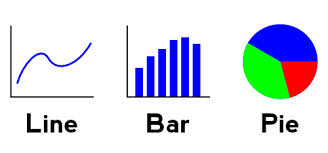
\includegraphics[scale=0.5]{charts2}
\end{center}
Most spreadsheets include \textbf{database functions} which can be used to
treat a table in the spreadsheet as if it were a database.
\subsection{Databases}
A \textbf{database} is a collection of related data, and the software used in
databases to store, organize and retrieve the data is called the \textbf{database
management system}, or \textbf{DBMS}. However, we often use the word \textsl{database}
to cover both meanings. A database can manage any type of data, including text, numbers, images,
sound, video and hyperlinks (links to websites).\\
Information is entered into the database via \textbf{fields}. Each field holds a separate piece of
information, and the fields are grouped together in \textbf{records}. Therefore, a record
about an employee might consist of several fields which give their name, address, phone number,
date of birth, salary and length of employment with the company.\\
Records are grouped together into \textbf{files} which hold large amounts of information.
Files can easily be \textbf{updated} - you can always change fields, add new records
or delete old ones. An electronic database is much faster to consult and update
than a card index system and occupies a lot less space. With the right software,
you can keep track of stock, sales, market trends, orders and other information
that can help your company stay successful.\\
A database program lets you create an \textbf{index} - a list of records
ordered according to the content of certain fields. This helps you to \textbf{search}
the database and \textbf{sort} records into numerical or alphabetical order very quickly.
Modern database are \textbf{relational} - that is, they are made up of
related files: customers and orders, vendors and purchases, students and tutors, etc.
Two database files can be related as long as they have a common field. A file
of students, for example, could include a field called \textsl{TutorID} and another file
with details of the tutors could include the same field. This \textbf{key field} can be used
to relate the two files. Databases like Oracle, DB2 and MySQL can manage these relatioships.\\
A database \textbf{query} function allows you to extract information according to certain
conditions or criteria. For example, if a managing director wanted to know all the
customers that spend more than \EUR8,000 per month, the program would search
on the name field and the money field simultaneously.\\ The best database packages
also include \textbf{network} facilities, which can make businesses more productive.
For example, managers of different departments can have direct access to a common database.
Most aspects of the program can be protected by user-defined passwords and other
\textbf{security devices}. For example, if you wanted to share an employee's
personal details but not their commission, you could protect the commission field.
\subsection{Email}
When you set up an account with an Internet Service Provider, you are given an
\textbf{email address} and a \textbf{password}. The mail you receive is stored on
the \textbf{mail server} of your ISP - in a simulated mailbox - until
you next connect and download it to your hard drive.\\
There are two ways to get email over the Internet. One is by using a \textbf{mail program}
(known as an \textbf{email client}) installed on your computer, for example Thunderbird or
Outlook Express. The other way is to use \textbf{web-based email}, accessible from any
web browser. Hotmail and Gmail are good examples.\\
You can make the message more expressive by including \textbf{emoticons}, also called
\textbf{smileys}. For example, ;-) for wink, :-) for happy, :-o for surprised, :-D for
laughing, etc. You may also like to add a \textbf{signature file}, a pre-written text file
appended to the end of the message. The name given to unsolicited email messages is \textbf{spam}.
\subsubsection{The anatomy of an email}
An email \textbf{address} (for example \emph{dexter@killer.com}) is made up of:
\begin{itemize}
\item a \textbf{username}, the name or nickname of the recipient (in this case, \emph{dexter})
\item the @ sign, which means \emph{at}
\item the \textbf{domain name \textnormal{or} network address} (in this case \emph{killer.com})
that is, the mail server where the account is located. The final part adds information about it, for example
com = company, uk = United Kingdom, it = Italy
\end{itemize}
An email \textbf{header} is made up of:
\begin{itemize}
\item \textbf{To line}: name and address of the recipient
\item \textbf{From line}: name and address of the sender
\item \textbf{Cc line}: carbon copy sent to another person
\item \textbf{Bcc line}: blind carbon copy (the recipient can't see other recipients' addresses)
\item \textbf{Subject}: topic of the message
\item \textbf{Attachment}: files added to the message
\end{itemize}
The \textbf{body} contains the message itself.
\newpage
\section{Acronyms and Keywords}
\begin{itemize}
\item CPU central processing unit
\item MODEM modulator and demodulator
\item PC personal computer
\item OS operating system
\item RAM random access memory
\item CD compact disc
\item CD-ROM compact disc read only memory
\item DVD digital versatile disc
\item LCD liquid crystal display
\item IT information technology
\item ICT information communication technology
\item PIN personal identification number
\item WWW world wide web
\item ISP internet service provider
\item HTML hypertext markup language
\item HTTP hypertext transfer protocol
\item SMS short message system
\item SIM subscriber identity module
\item MMS multimedia messages
\item FAQ frequently asked question
\item CLI command line interface
\item UI user interface
\item GUI graphical user interface
\item DBMS database management system
\item RDBMS relational database management system
\item SQL structured query language
\item \textbf{multiuser} allows many users to use a computer at the same time 
\item \textbf{multitasking} allows the user to run several programs at the 
same time
\item \textbf{open source} the source code is freely available and everybody
can read and modify it
\item \textbf{window} variable-sized rectangle ued to display information
\item \textbf{pointer} is an arrow that can be moved around the screen and
is used to select things
\item \textbf{device driver} is a program that allows a hardware device,
such as a printer, to communicate with a computer
\item a \textbf{relational database} has more than one table and the tables are linked using key fields
\item in a database, a \textbf{field} stores a single piece of information
\item a database \textbf{record} consists of a number of interrelated data elements, called fields
\item a \textbf{key field} is a field in a record that holds unique data which identifies that record from all the 
other records in the file or database
\item a database \textbf{report} presents information from a database. It can be printed from the database
to view information quickly and easily 
\item an \textbf{index} is a list of records ordered according to the content of certain fields 
\end{itemize}
\end{document}
